\documentclass{article}

\usepackage[utf8]{inputenc}
\usepackage[T1]{fontenc}
\usepackage[greek,english]{babel}
\usepackage{alphabeta}
\usepackage{amsmath}
\usepackage{amssymb}
\usepackage{graphicx}
\usepackage{subcaption}
\usepackage{epstopdf}
\usepackage[margin=1in, paperwidth=7.5in,paperheight=10.5in]{geometry}
\usepackage{hyperref}
\usepackage{paracol}

\newcommand\course{ΗΡΥ 411}
\newcommand\courseName{Ενσωματωμένα Συστήματα Μικροεπεξεργατών}
\newcommand\semester{Χειμερινό 2020-2021}
\newcommand\assignmentNumber{Εργαστήριο 3}
\newcommand\studentName{Μαυρογιώργης Δημήτρης}                           
\newcommand\studentNumber{2016030016}

\title{\underline{\textbf{\assignmentNumber}}} 
\author{\textsc{\textbf{Όνομα:}}  \studentName\\
		\textsc{\textbf{ΑΜ:}}  \studentNumber\\
		\course \ - \courseName\\ 
		\textsc{Πολυτεχνείο Κρήτης}
		}
\date{\today}
\begin{document}
	\maketitle

\section*{Σκοπός}
	Σκοπός του τέταρτου εργαστηρίου είναι να υλοποιήσουμε σε κώδικα C τις αρχικοποιήσεις των TIMER0 και USART, κρατώντας αυτούσιους τους κώδικες των interrupt handler που είχαν υλοποιηθεί στο εργαστήριο 2 και 3 αντίστοιχα. Στόχος μας είναι, δηλαδή, να συνδυάσουμε τον κώδικα C των αρχικοποιήσεων και του κώδικα assembly των handler προκειμένου να υλοποίησουμε τις προδιαγραφές που είχαν περιγραφθεί στα δύο προηγούμενα εργαστήρια.

\section*{Περιγραφή της υλοποίησης}
	Στο συγκερκιμένο εργαστήριο οι αλλαγές που χρειάστηκε να γίνουν είναι να κάνουμε τις αρχικοποιήσεις των δύο handler σε C και στη main του προγράμματος να χρησιμοποιήσουμε ένα infinite loop. Eιδικότερα, οι αρχικοποιήσεις των τιμών των καταχωρητών είναι ακριβώς ίδιες μου του προηγούμενου εργαστηρίου. Οι αρχικοποιήσεις αυτές έγιναν σε δύο ξεχωριστές συναρτήσεις και το μοναδικό που αλλάζει είναι ότι καλούνται στο main πρόγραμμα.\\
	
	\noindent
	Όσον αφορά τον κώδικα assembly, η υλοποιήσεις των handler είναι η ίδια με του εργαστηρίου 3, με μοναδική αλλαγή τη μετονομασία τους από TIMER0\_OVF και USART\_RXC σε \\ TIMER0\_OVF\_vect και USART\_RXC\_vect αντίστοιχα. Oι συγκεκριμένοι handler, \\ δηλώθηκαν ως global για να μπορούν να αναγνωριστούν από τη C.\\
	
	\noindent
	Παράλληλα, δηλώθηκε και η συνάρτηση MEM\_INIT ως global, για την αρχικοποίηση των X και Y registers έτσι, ώστε να κρατούν τις διευθύνσεις των array που είναι αποθηκευμένες οι αποκωδικοποιήσεων των αριθμών για τα 7-segment και τα δεδομένα προς εμφάνιση αντίστοιχα.\\
	
	\noindent
	Κατόπιν, για να είναι σβησμένα τα 7-segment display, έγινε ένα clear της μνημης με τη συνάρτηση MEM\_CLEAR, δηλαδή αποθηκεύτηκαν και στις 8 θέσεις το 0x0A. Για να μπορέσουμε να καλέσουμε και αυτή τη συνάρτηση στη C, δηλώθηκε και αυτή ως global. Τέλος, όλες οι δηλώσεις με .equ των γραμμάτων των εντολών, που δηλώθηκαν στην assembly του 3ου εργαστηρίου, έγιναν με \#define. \\
	
	\noindent
	Παρακάτω φαίνονται οι κώδικες C και οι αλλαγές του κώδικα Assembly, όπως περιγράφτηκαν προηγουμένως.
\pagebreak
	\begin{figure}[h!]
		\centering
		\begin{subfigure}[t]{0.5\textwidth}
			\centering
			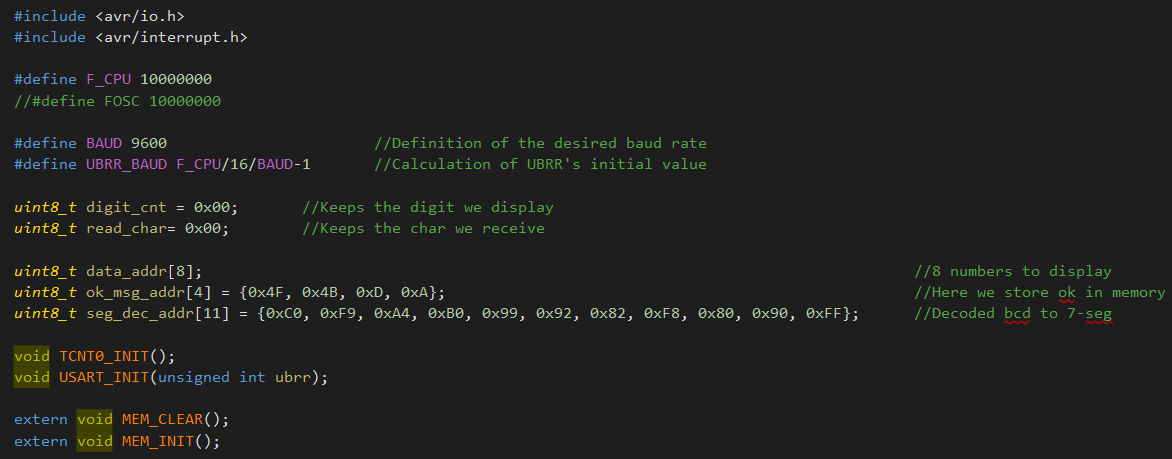
\includegraphics[height=3.5cm, width=\linewidth]{./results/lab4_defines.png}
			\caption{C code for defines global variables and function signatures}
		\end{subfigure}%
		~
		\begin{subfigure}[t]{0.5\textwidth}
			\centering
			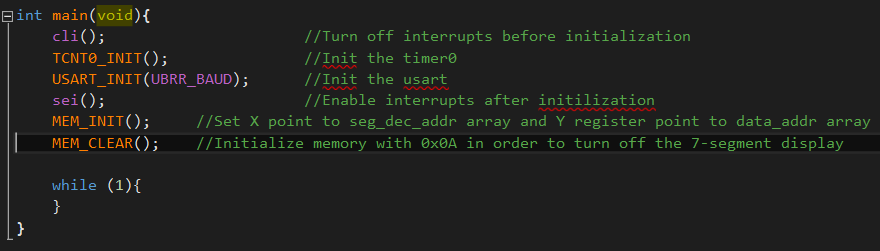
\includegraphics[height=3.5cm, width=\linewidth]{./results/lab4_main.png}
			\caption{C code for main}
		\end{subfigure}
	
		\begin{subfigure}[t]{0.5\textwidth}
			\centering
			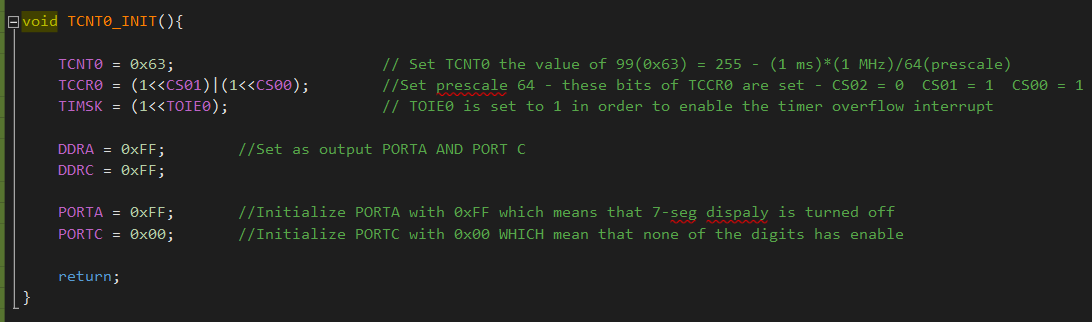
\includegraphics[height=3.5cm, width=\linewidth]{./results/lab4_time0_init.png}
			\caption{C code for TIMER0 Initialization}
		\end{subfigure}%
		~
		\begin{subfigure}[t]{0.5\textwidth}
			\centering
			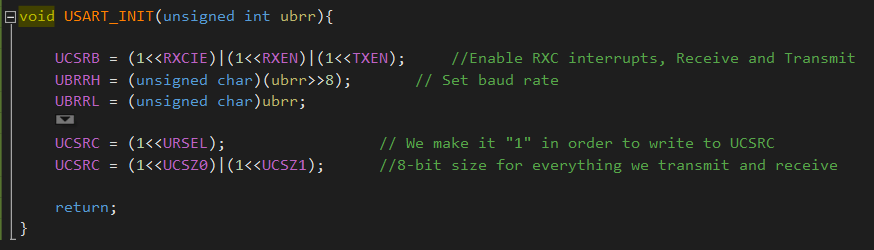
\includegraphics[height=3.5cm, width=\linewidth]{./results/lab4_usart_init.png}
			\caption{C code for USART RXC Initialization}
		\end{subfigure}	
	
		\begin{subfigure}[t]{0.5\textwidth}
			\centering
			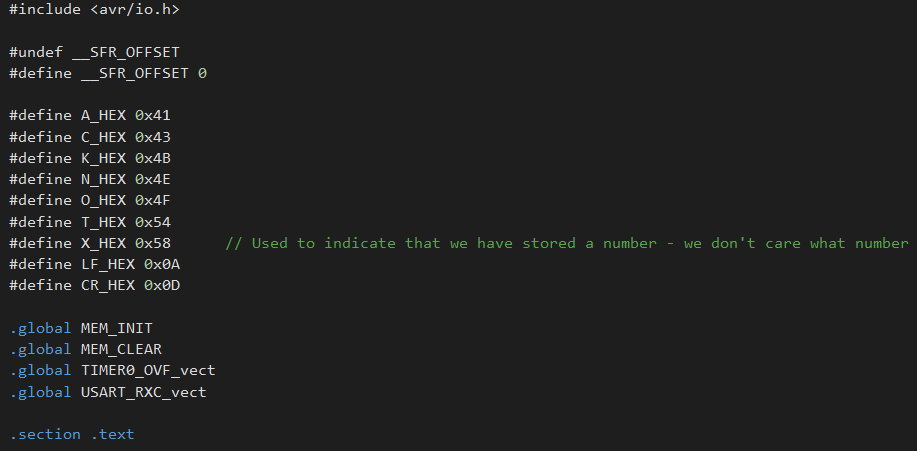
\includegraphics[height=3cm, width=\linewidth]{./results/lab4_assembly_changes.png}
			\caption{Assembly code changes}
		\end{subfigure}	
	\end{figure}
	
	\noindent
	Οι προσομοιώσεις του συγκεκριμένου εργαστηρίου είναι ακριβώς ίδιες με του προηγούμενου, εφόσον δεν έγιναν καθόλου αλλαγές στην υλοποίηση των TIMER0 και USRART handler. Eιδικότερα, στις παρακάτω εικόνες φαίνεται ότι γίνεται σωστά το initialization των καταχωρητών του TIMER0 και USART, καθώς και η αποθήκευση των αποκωδικοποιήσεων για τα 7-segment και του μηνυματος OK<CR><LF>. Eπίσης, βλέπουμε ότι εκτελείται σωστά ο USART handler και οι τιμές οι οποίες λαμβάννται αποθηκεύονται στη μνήμη, ενώ παράλληλα φαίνεται ότι εκτελείται σωστά και ο TIMER0 handler. Tέλος, όσον αφορά την αποστολή του OK<CR><LF>, μετά τη λήψη των αριθμώ, γίνεται η εγγραφή του στο αρχείο lab4.log, γεγονός που επιβεβαιώνει τη σωστή λειτουργία.\\
	
	\begin{figure}[h!]
		\centering
		\begin{subfigure}[t]{0.5\textwidth}
			\centering
			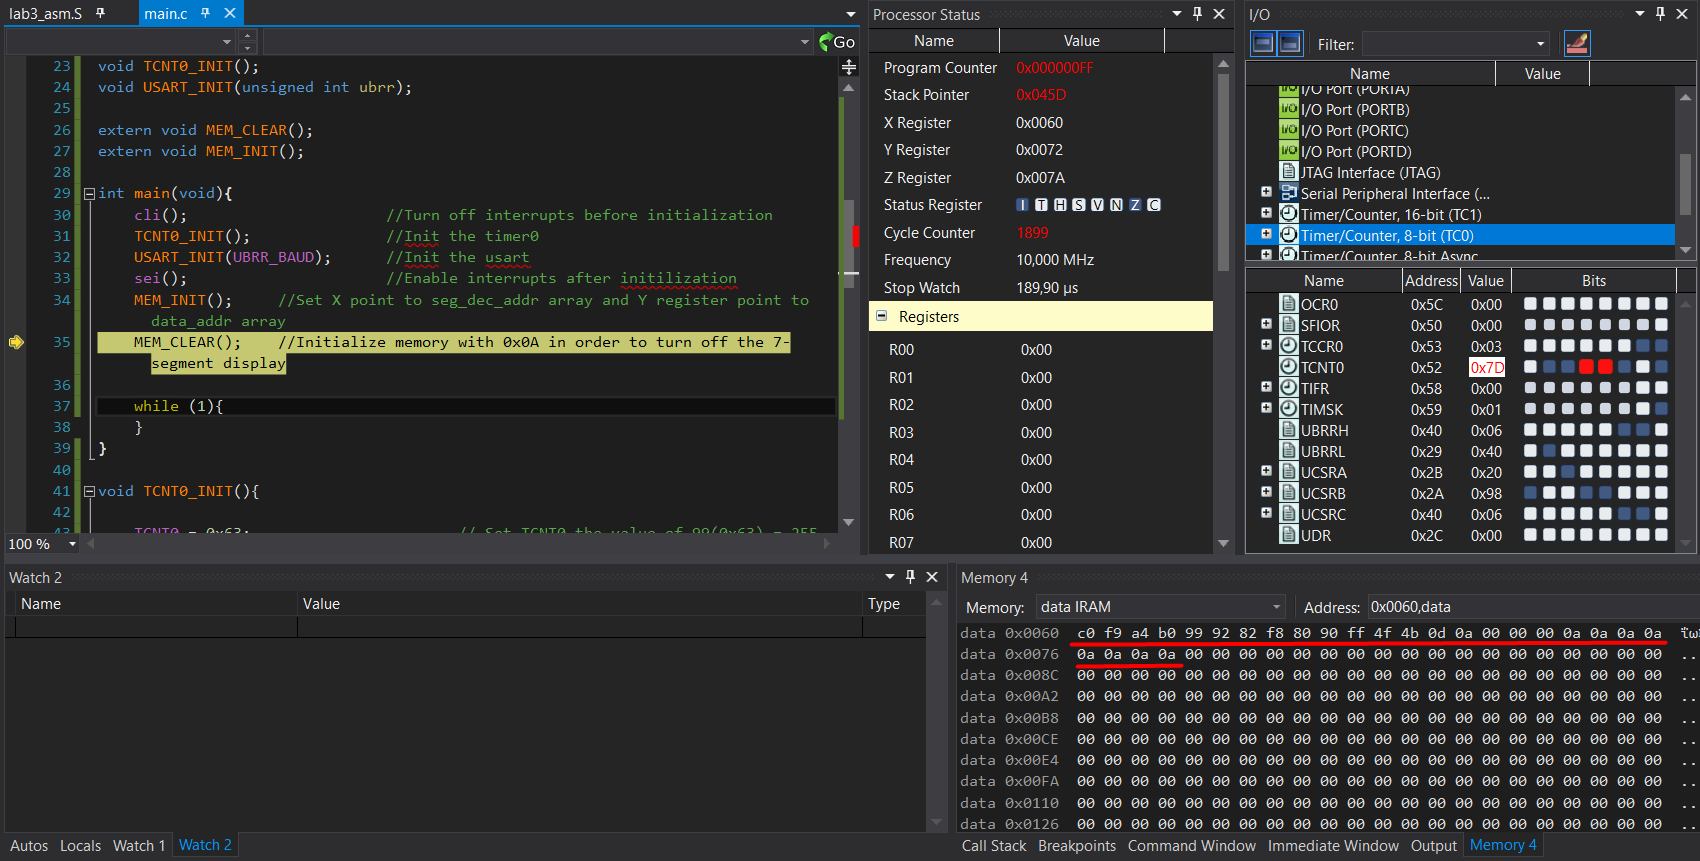
\includegraphics[height=3.2cm, width=\linewidth]{./results/lab4_sim_init.png}
			\caption{Αtmel Studio 7 - Initialization of TIMER0 and USART}
		\end{subfigure}%
		~
		\begin{subfigure}[t]{0.5\textwidth}
			\centering
			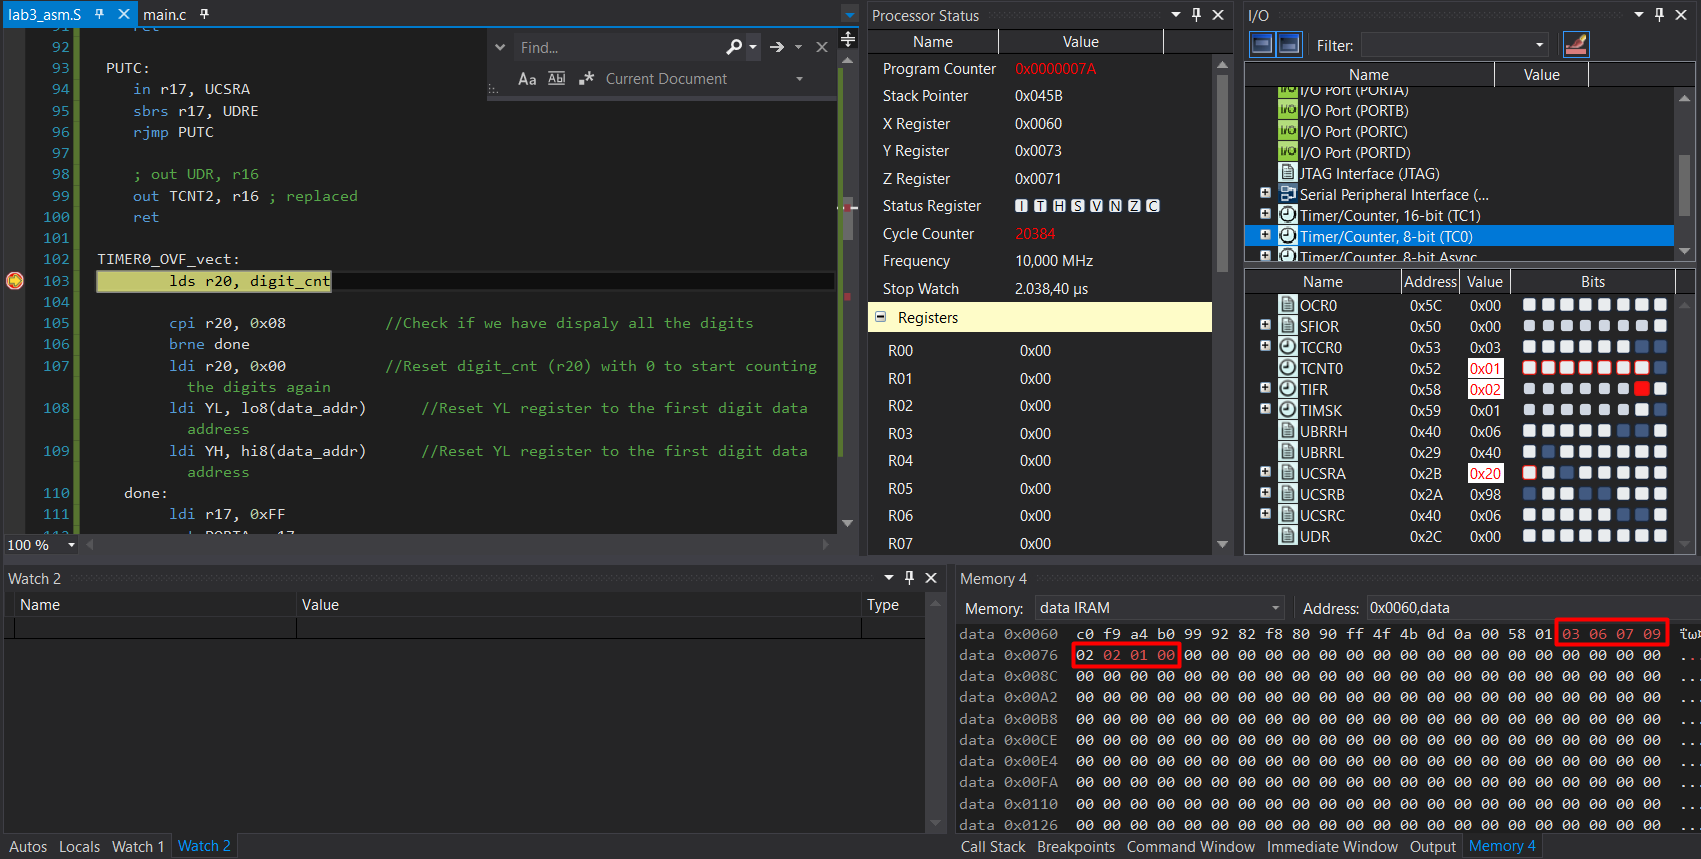
\includegraphics[height=3.2cm, width=\linewidth]{./results/lab4_sim_num.png}
			\caption{Αtmel Studio 7 - Execution of N01229763<CR><LF>}
		\end{subfigure}
	\end{figure}

\pagebreak
\noindent
	Επιπρόσθετα, κατα την προσομοίωση του κώδικα C, μπορούμε να δούμε τον κώδικα Assembly που δημιουργήθηκε για τις αρχικοποιήσεις. Όπως φαίνεται παρακάτω ο κώδικας αρχικοποίησης σε assembly του 3ου εργαστηρίου και ο κώδικα που δημιούργησε ο compiler είναι παρόμοιοι, με μικρές διαφορές. Οι κυριότερες διαφορές είναι ότι τα ονόματα των καταχωρητών μεταφράστηκαν στις διευθύνσεις τους και μία άλλη αλλαγή είναι ότι χρησιμοποιούνται διαφορετικοί καταχωρητές (πχ στο 3ο Lab είχε χρησιμοποιηθεί για τον TIMER0 ο R16, ενώ στο συγκεκριμένο Lab χρησιμοποιείται ο R24).
	
	\begin{figure}[h!]
		\centering
		\begin{subfigure}[t]{0.5\textwidth}
			\centering
			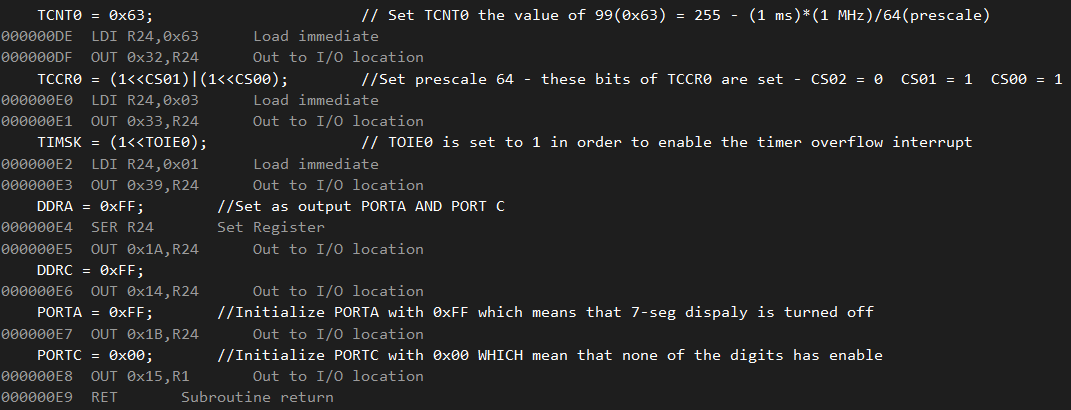
\includegraphics[height=3.2cm, width=\linewidth]{./results/lab4_c_to_assembly_timer0_init.png}
			\caption{Assembly generated code for TIMER0 initialization}
		\end{subfigure}%
		~
		\begin{subfigure}[t]{0.5\textwidth}
			\centering
			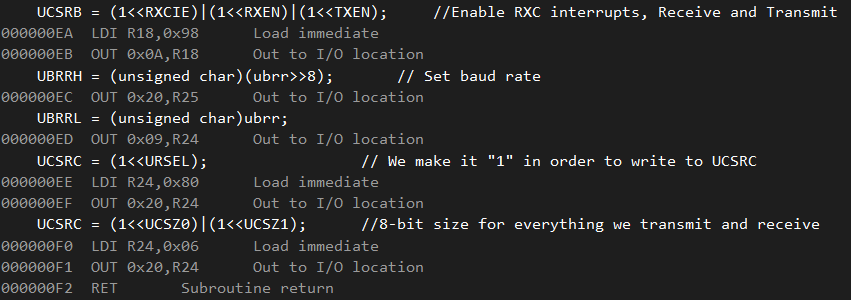
\includegraphics[height=3.2cm, width=\linewidth]{./results/lab4_c_to_assembly_usart_init.png}
			\caption{Assembly generated code for USART initialization}
		\end{subfigure}
	\end{figure}
\end{document}
